% !TEX root = thesis.tex

\chapter{Simulations}
\label{ch:simulations}

Numerical simulations have emerged as a new tool to investigate nature, alongside theory and experiments.
This is particularly valid for astronomy where, unlike other laboratory-based disciplines, astronomers may not exert full control over their experiments \citep{Heng2014}.

Computer simulations are essentially a tools to solve complex systems of equations which are intractable with analytic techniques, or only tractable with very coarse level of approximation \citep{Springel2016}.
This allows an unprecedented detailed exploration of the consequences of assumed models for physical systems. In this sense, the reproduction of observations through computer simulations is a way to validate scientific hypotheses.
The main mathematical model used in galaxy simulations is the fluid model, a branch of continuum mechanics which deals with materials represented as continuous mass as opposed to discrete particles.
% The main assumption of this is that particles... \citep{Vandenbroucke2016}.
In the following we will be dealing with hydrodynamics of fluids, given that the main components of galaxies are successfully described in terms of fluids.

\section{Hydrodynamics}

\subsection{Boltzmann Equation - Equations of motion}
% We will assume that dark matter consists of small particles that are orders of magnitude smaller than the typical distance scales in our galaxies, so that we will treat it as a collisionless fluid.
% SPH The main assumption SPH can be used to solve the 
% The equation of hydrodynamics are derived from the Boltzmann equation.
This equation is generally valid for any type of fluid, also for a collisionless fluid.
The direct numerical solution of the CBE, a non-linear PDE in seven dimensions, is not feasible.
% In this case we can solve the Boltzmann equation directly, by using characteristic solutions.
To this end, we represent the collisionless fluid by $N$ mass elements (particles).
In practice an $N$-body method is a tool for solving the collisionless Boltzmann equations.
% In this way then it reduces to solving the gravitational interactions for this $N$-body system \citep{Dehnem2011}.

At any given time, it is possible to fully describe an $N$-body system (a set of particles with equal mass $m$) by its distribution function $f(\vect x, \vect v, t)$ which represents the number density of particles in the 6D phase space $(\vect x, \vect v)$. By multiplying this function with the phase space volume element $\d{\vect x} \d{\vect v}$, we obtain the number of particles within this phase space volume element at a given time $t$.
The number density $n$ in physical space is obtained by integrating over the velocity:
\begin{equation}
n(\vect x,t ) = \int f(\vect x, \vect v, t) \d{\vect v}.
\end{equation}
The spatial density is then simply $\rho=mn$.

Collisionless Boltzmann equation (a.k.a. Vlasov equation).
\begin{equation}
...
\end{equation}

\section{N-Body systems}
% It is interesting to note that in this description the particles have basically completely vanished and have been replaced with a continuum fluid description. Later, 
For the purpose of solving the equations, the main idea is to discretize the equations above introducing paritcles. These are then not the real physical particles any more, rather they are fiducial macro particles that sample the phase-space in a Monte-Carlo fashion \citep{Springel2016}.


\subsection{Smoothed Particles Hydrodynamics}
Smoothed Particles Hydrodynamics (SPH) is a finite volume, lagrangian particle based numerical method to solve the Navier-Stokes equation of motions for a fluid.
It is a lagrangian method because the elements carrying information about the fluid move along the fluid itself.
% It is finite volume because it.

A different approach to discretize the fluid domain is to use Eulerian approach, like grid based Adaptive Mesh Refinement (AMR).
Recently, so called \emph{moving-mesh} methods have emerged. They combine both approaches and are more flexible but come with their own difficulties \citep{Springel2010, Shadowfax, Arepo}.
% Several research groups are pushing forward different techniques, sometimes following their own tradition and claiming. 
Usually simple test problems (Sod tube (1D,2D), Sedov blast, Kelvin-Helmholtz instabilities, Noh test, Gresho vortex \citet{Gresho1990}), %TODO fix test
which can be solved analytically, serve as a benchmark for the accuracy of the numerical solution, \citep[e.g. by measuring the distance of the two solution with an L2-norm in the whole domain, ][]{BorrowSphenix}.
Numerical solutions are always a tradeoff between the accuracy and the practicality.
It is interesting to see how a certain gain in accuracy is translated in an increase of \emph{time-to-solution}.
%But at the end of the day if we pay attention to the the trend is 

SPH has been originally developed as a \emph{probabilistic} particle method for simulating astrophysical problems \citep{Lucy1977, Gingold1977}\footnote{In a lecture given at Monash University in 2018 \url{https://youtu.be/tAXHCAEgSuE}, prof. Joe Monaghan retrace the origin of the SPH method, recalling that the inspiration for the particle methods to estimate density in fluids comes from David George Kendall, a statistician he collaborated with in Cambridge.}.

% In his original treatment \citet{Gingold1977} the probabilities of ... were defined as the expected value
% \begin{equation}
%  E[\rho] = ...% TODO expected values
% \end{equation}

% From J. Monaghan https://www.youtube.com/watch?v=tAXHCAEgSuE
% The general procedure of SPH for solving equations is:
% \begin{itemize}
%  \item Replace the continuum by particles
%  \item Calculate forces on particles
%  \item Follow the motion of the particles
% \end{itemize}
% In statistics the basic interpolant is used to compute probability density except that they do not have mass.
% Instead, for $N$ samples they have the factor $\frac 1 N$.



% Cambridge David Kendall professor of statistics they wanted to calculate probability distributions from samples. They use the same kind of interpolation.

% Problems: Accessing particles (if you have gravity the tree that you build to compute distances and gravity interactions between all the particles can be used in hydrodinamics too.
% The hydro differential equations become a set of ordinary differential equations and (t42:00) and a way to  timestepping is needed.
% Try to construct your discretized equations in a way that it contains the conservation properties of the continuum.

\section{Density Estimation from particles ensemble}
A possible choice for the kernel is a Gaussian.
% TODO kernel
It's much more practical to use a finite support approximation of a Gaussian.
The most used for SPH are the Schoenberg  B-spline functions \citep{Schoenberg1988}, generated as the Fourier transform \citep{Price2012}:
\begin{equation}
M_n(r, h) = \frac{1}{2\pi}\int_{-\infty}^{\infty}{\left(\frac{\sin(kh/2)}{kh/2}\right)^n\cos(kr)\d k}.
\end{equation}

By increasing $n$ we obtain progressively better approximations to the Gaussian. It is convenient to require continuity in at least the first and second derivatives, so the lowest order and most widely used B-spline useful for SPH is the cubic spline kernel $M_4$:
\begin{equation}
M_4(q) = \frac{1}{\pi h^3} \left\{
\begin{array}{ll}
\frac{1}{4}(2-q)^3 - (1 - q)^{3}, & 0 \le q < 1; \\
\frac{1}{4}(2-q)^3, & 1 \le q < 2; \\
0. & q \ge 2,
\end{array}
\right.
\label{eq:cubicspline}
\end{equation}
where $q=r/h$ is the distance normalized by the smoothing length.

\paragraph{Role of the normalization term}
% TODO probabilistic treatment if it fits
It is somehow striking that the normalization term is not the default in current visualization routines, the only reason being spurious effects when dealing with free surfaces \citep{Price2007}.

\begin{equation}
 A(\vect r) = \dfrac{\sum_j \frac{m_j}{\rho_j} A_j W(|\vect r - \vect r_j|,h)}{\sum_j \frac{m_j}{\rho_j} W(|\vect r - \vect r_j|,h)}.
\end{equation}
...

\section{Dwarf galaxies models}
\citet{Verbeke2017}
\subsection{Gravity}
\subsection{Hydrodynamics}
\subsection{Sub-grid models}
For a review see \citet{Verbeke2017, Vandenbroucke2016}.

\paragraph{Star Formation}
Star particles are formed in converging, cold and dense regions of gas.
The following three conditions must be true for a gas particle to be eligible to become a star particle.
\begin{align*}
 T_g &< 15000 \text{~K},\\
 \rho_g &> 100 \text{~amu~cm}^{-3},\\
 \nabla \cdot \vect v & < 0.
\end{align*}

The conversion into star particles of gas particles which meet the above conditions is governed by a Schmidt relation \citep{Schmidt1959}
\begin{equation}                                                                              
\dot{\rho}_\star = -\dot{\rho}_g = c_\star \frac{\rho}{t_g}.
\label{eq:schmidt_relation}
\end{equation}
Following \citep{Stinson2006} we assume the characteristic time of formation as the dynamical time $t_g = (4 \pi G \rho_g)^{-1/2}$, whereas $c_\star$ is the star formation efficiency which can be adjusted to match observations.

From this, we can solve the simple differential equation: 
\begin{equation}
\rho_\star = 1 - e^{c_\star \frac{t}{t_g}}.
\end{equation}
We can then use a stochastic method to determine if an eligible gas particle has to be turned in a gas particle.
The Monte Carlo threshold probability of star formation event:
\begin{equation}
P_\star = 1-\exp(-\frac{c_\star \delta t}{t_g}),
\end{equation}
where $\delta t$ is the integration time step.
Given a random number $X \in \mathcal{U}(0,1)$ a star can form if $X < P_\star$.
Several authors \citep{Stinson2006, Cloet-Osselaer2012, Revaz2009} have pointed out that since the star formation is a self-regulating process the star formation rate is weakly dependent on the the choice of $c_\star$ above $0.1$. In our case we use $c_\star = 0.25$.
The new star particle inherits the position, velocity and metallicity of its gas particle progenitor.
In all effects, star particles represent a stellar population with single age and metallicity (SSP, Single Stellar Population) with a Chabrier initial-mass function, \citet{Chabrier2003}.

\paragraph{Stellar feedback}
By \emph{feedback mechanism} it is meant any process that allows to exchange energy, matter and/or momentum between galaxy components. Stars have a huge influence on the interstellar medium (ISM), they pump energy and matter in the surrounding gas mainly enriching ISM with newly formed metals.

The first type of feedback comes from supernovae events. Two main supernovae type are important in simulations. For massive stars, when all the fusion fuel is consumed, gravitation overcome the internal hydrodynamic pressure. The core of the star collapses generating a shock wave which blows away most of the star's outer atmosphere in a massive explosion, leaving behind only a small fraction of its mass, locked up in a remnant (a neutron star or a black hole). This type of core-collapse supernova is called \snii{} (type II supernova).
This type of feedback lasts from the death of the most massive stars of the sampled by the particle's SSP, until the death of the least massive stars which are still capable of going supernova ($>8$ \Msun ): $0.005 - 0.043$ Gyr.
For less massive stars, Type~Ia supernova occurs in a binary star system made by a red giant and a white dwarf.
The gas from a red giant overflows onto a white dwarf and when a critical mass is reached, the white dwarf can no longer be supported and collapses, then rebounds. Neutrinos are thought to play an important role in this expansion \citep{Wongwathanarat2017}.
Because it involves less massive stars and demands a period of steady accretion the feedback of \snia{} is returned $1.54 − 1.87$~Gyr after the birth of the star particle. Energy injection of \snia{} is delayed by a normally distributed offset-time following \citet{Strolger2004}.
Feedback from supernovae events of type Ia (\snia) and II (\snii) inject $10^{51}$~erg into the surrounding ISM. For more details, the reader is referred to \cite{Valcke2008}.

% Adapted from Simon Driver
%Ia vs Ib depends on if the companion has hydrogen in the atmosphere.

Supernovae events increase the metal content of the ISM. %tracked by Fe and Mg element abundances in gas particles.
In simulations these effects are taken into account by keeping track of two independent metallicities:\feh, \mgfe, corresponding to a fast contribution by the supernova explosions of massive stars, and a slow contribution by the supernova explosions of less massive stars \citep{DeRijcke2013, Vandenbroucke2016}.

A second type type of feedback is stellar wind from young O and B stars.
In simulation stellar wind is taken into account as a uniformly spread energy injection of $10^{50}$ erg in the ISM for $31$~Myr, i.e. from the birth of the star particle until the last massive star ($m = 8$~\Msun) turns \snii{}.


% The stellar population in the star particle is modelled by an initial mass function which tells how many stars are formed with a certain amount of mass. 

\subsection{Extended gas physics}
\paragraph{Radiative cooling}

\paragraph{Ionization aware equation of state}
In an ideal gas with a single type of constituents, the pressure is given by the equation of state:
\begin{equation}
p = n k_B T
\end{equation}

From \citep[p. 161]{Vandenbroucke2016}, in a multiphase, multicomponent gas with species $S$, this becomes:
\begin{equation}
p = \left(\sum_S n_s + n_e(T)\right) k_BT =\frac{\rho k_B T}{\bar\mu}
\end{equation}
where we introduced the mean constituent mass $\bar\mu$ which is precomputed and tabulated as a function of $\bar\mu = \bar\mu(T, \feh, \mgfe, z, \rho)$.

\subparagraph{Modified equation of energy when considering ionization}
We assume a gas of ${}^1$H with an ionization fraction $x$.
We consider the internal energy to be composed by a (thermal) kinetic part and a ionization part:
\begin{equation}
\label{eq:u}
u = u_\text{kin} + u_\text{ion}
\end{equation}
The kinetic term (directly linked with the temperature) is defined as
\begin{equation}
u_\text{kin} = \frac 3 2 k_B T/ \mu, 
\end{equation}
whereas the ionization energy is
\begin{equation}
\label{eq:u_ion}
u_\text{ion} = \dfrac{\chi_\text H}{m_\text H} x,
\end{equation}
with $\chi_\text H$ and $m_H$ the ionization energy and atomic mass of ${}^1$H.

Assuming no temporal composition changes in the gas (i.e. assuming the gas in ionization equilibrium), the ionization fraction is a function only of the temperature (i.e. the internal kinetic energy) $x = x(T) = x(u_\text{kin})$, which allows the temporal derivative of equation \eqref{eq:u_ion} to be written as:
\begin{equation}
\label{eq:du_ion}
\dv{u_\text{ion}}{t} = 
\frac{\chi_\text H}{m_\text H} \dv{x}{u_\text{kin}} \dv{u_\text{kin}}{t}
\end{equation}
From equations \eqref{eq:u} and \eqref{eq:du_ion}:
% \begin{equation}
% \dv{u_\text{kin}}{t} = \dv{u}{t} - \frac{\chi_\text H}{m_\text H} \dv{x}{u_\text{kin}} \dv{u_\text{kin}}{t}
% \end{equation}
\begin{equation}
\dv{u}{t} = \dv{u_\text{kin}}{t} \left( 1+\frac{\chi_\text H}{m_\text H} \dv{x}{u_\text{kin}}\right).
\end{equation}
By defining $X_\text{ukin} = \frac{\chi_\text H}{m_\text H} \dv{x}{u_\text{kin}}$,
the energy equation is then:
\begin{equation}
\dv{u}{t} = \dfrac{1}{ 1 + X_\text{ukin}} \dv{u_\text{kin}}{t}
\end{equation}

Instead of evolving the total thermal energy, we can hence evolve the kinetic thermal energy, and adapt the thermal energy equation by applying the correction term $X_\text{ukin}$.
This can be precomputed and tabulated as a function of $(T, \feh, \mgfe, z, \rho)$.

\paragraph{Ultraviolet background}
UV background is implemented and varies with redshift following the model by \citet{Faucher-Giguere2009}.


\subsection{Moving box}

Using SPH it is computationally challenging to simulate an entire cluster of hot gas while at the same time having the resolution to properly treat the interactions at the interface between the interstellar and intra-cluster medium (or ICM) that cause ram pressure stripping.

We have opted to use the moving-box technique described by \citet{Nichols2015} and further developed by \citet{Hausammann2019}.
We enclose the MoRIA dwarf in a $60$~kpc wide moving simulation box, as in a wind tunnel simulation.
Gas is injected from the open "front" side of the box, which always points in the dwarf's direction of motion. Its density and temperature vary with position, as discussed below. This mimics the hot wind of the cluster halo gas as it streams past the orbiting dwarf galaxy.
Also, additional fictitious forces on the particles are included to take into account the rotation and orbital motion of the moving box.
This allows us to simulate the combined effects of tidal forces and ram-pressure stripping \citep[as studied by][]{Mayer2006} which are acting simultaneously on the dwarf without the necessity of simulating a galaxy cluster worth of intra-cluster gas.
A slight improvement in our implementation of the moving-box method is the use of a critically damped oscillator for the \emph{ad~hoc} acceleration to keep the galaxy close to the centre of the box.
A typical simulation snapshot contains around $150$k gas particles and $16$k star particles, each with a mass of $4000$~\Msun{}.

\paragraph{Reference frames} In a moving box simulation, reference frames have an inportant roles.
We define the inertial reference frame where the cluster is at the origin.
Relative to that the box moves and rotates.
To represent the correct rotations, the moving box is 


\subsection{Recovering the correct kinematics from a moving box simulation}
\label{sec:corret_kinematics}
Following the convention in \citet{Nichols2015}, capital letters are used for vectors in the inertial frame whereas small letters for vectors in the moving box (rotating frame).
Let $\vect \Omega$ be the angular velocity of the box in the inertial frame, and $\mathbf q$ the quaternion which at each point in time maps the $-y$ axis of the rotating reference frame to the direction of the velocity of the box in the inertial frame, $\Vp$.
A vector $\vect X$ in the inertial frame, corresponds to $\vect x = \mathbf q^{-1}\, \vect X \,\mathbf q $ in the rotating frame.

The velocity of the box is measured using a fixed point inside the box, called \emph{pivot}, whose coordinates relative to the box are $\mathbf{x}_{\mathrm p}$ and its velocity and acceleration in the inertial frame relative to the cluster are denoted with $\Vp$ and $\Ap$, respectively.
The \emph{pivot} represents the position in the box of minimal specific energy at the start of the simulation \citep{Hausammann2019}.
From this, $\vect \Omega$ can be computed as 
\begin{equation}
 \vect{\Omega} = {(\Vp\times\Ap)}/{\Vp^2}
\end{equation}
and the angular velocity of the box w.r.t. the rotating frame simply as:
\begin{equation}
\vect \omega = \mathbf q^{-1}\, \vect \Omega\, \mathbf q.
\end{equation}
We can then transform from rotating to inertial coordinates by applying this transformation:
\begin{equation}
\vect V = \Vp + \mathbf q \left(\mathbf v + \vect \omega \times (\mathbf x-\mathbf x_{\mathrm p})\right) \mathbf q^{-1}
\end{equation}
where $\mathbf x$ and $\mathbf v$ are position and velocity of the particle in the rotating frame, respectively, and $\mathbf V$ its velocity in the inertial frame. % For simplicity in the following we don't take into account $\Vp$ since its contribution to the line of sight velocity is negligible.


\section{Simulating the Fornax cluster environment}\label{sec:fornax_sim}

\subsection{Cluster model}

\subsubsection{Dark matter}
The simulations take into account both ram pressure stripping and the tidal interaction with the cluster.
The latter is simulated as a single spherically symmetric static NFW potential profile \citep{Navarro1996} with mass $M~=~10^{14}$~\Msun{} \citep{Drinkwater2001a}:
\begin{equation}
    \Phi(r) = \frac{G M}{r} \frac{\log(1+r/R_s)}{\log(1 + c) - \frac{c}{1+c}}
\end{equation}
with scale length $R_s = 120$ kpc and $c=8.15$ derived from scaling relations in e.g. \citet{Gentile2004, Wechsler2002}:
\begin{equation}
    c \simeq 20 \left(\frac{M}{10^{11} \text{\Msun{}} }\right)^{-0.13}, \qquad
    R_s = \frac 1 c \left(\frac{M}{\frac 4 3 \pi 200 \rho_c}\right)^\frac 1 3,
\end{equation}
with $\rho_c = 127.3$~\Msun{}~kpc$^{-3}$ the critical density of the universe at $z=0$ for a cosmology with Hubble constant $h=0.67$ and $\Omega_m = 0.31$ \citep{Planck2015}.
The cluster virial radius of the model is $R_{\mathrm{vir}} = c R_s = 978$~kpc.

\subsubsection{ICM} \label{sec:ICM}
Following \citet{Paolillo2002}, we use the superposition of three spherically symmetric beta-models, $\rho(r) = \rho_0 (1 + (r/r_0)^2 )^{-3\beta/2}$, to construct the gas density profile in the Fornax cluster, as shown in Figure \ref{fig:profiles}.
They identify three contributions to the hot gas distributions: a central component (dominating for $r<5''$), coincident with the optical galaxy NGC1399; a less dense and more extended galactic component ($50''<r<400''$); and a cluster component ($r>400''$).
We assume the gas to be in hydrostatic equilibrium with temperature $T(r)$ computed as:
\begin{equation}
   T(r) = \frac {m_p}{k_B \rho(r)} \int_r^\infty \rho(r') \frac{GM(r')}{r'^2} \mathrm{d} r'
\end{equation}
where $M(r)$ is the mass of the gas, stars and dark matter beyond radius $r$, $m_p$ is the proton mass, $G$ and $k_B$ the gravitational and Boltzmann constants.

\begin{figure}
\centering
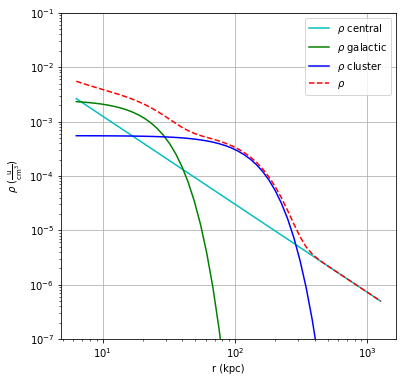
\includegraphics[width=0.8\textwidth]{PaolilloRho.png}
\caption{Gas density profile $\rho(r)$ of the  Fornax Cluster model as a superposition of three beta models from measurements described in \citet{Paolillo2002}, from which we also adopt the nomenclature for the different beta models.
}
\label{fig:profiles}
\end{figure}

These two radial profiles allow us to inject particles with the proper density and temperature in the moving box, hence recreating the environmental condition of the cluster as the dwarf orbits through it.

\subsection{Simulation parameters}
We carried out a set of simulations starting from five MoRIA models of late-type galaxies taken at $z = 0.5$.
The overall goal in setting up the simulations is to study the evolution of late-type galaxies in a cluster environment.
The choice of the redshift of infall has been motivated by the fact that the number of red dwarfs in the Fornax cluster has increased significantly since $z = 0.5$ \citep{Stott2007, DeRijcke2010}.
That indicates that the conversion of late-type to early-type dwarfs (and hence the acquisition of late-type dwarfs by clusters) is probably a recent event.

We selected dwarfs models covering the stellar mass range of $10^{7.5}-10^{9}$ and we injected each of them on 5 different orbits with pericenter distances of $50, 100, 150, 200,$ and $300$~kpc and with a fixed apocenter of 800 kpc.
The starting point of the infall is always at a radial distance of 600~kpc.
We chose a lower radial distance of the starting position w.r.t. the virial radius given the very low cluster density in that region and the low orbital velocity of the dwarf near apocentre.
In this way, simulations could be concentrated on the infall and the pericenter passages of the simulated dwarfs.
We evolved the galaxies for $5.5$~Gyrs up to $z=0$.
The initial stellar masses are reported in Table \ref{tbl:sim}. All simulations presented in this paper, at time of injection have exponentially declining SB profiles with Sersic index around 1.0.
Every $10$~Myr a snapshot is saved, yielding around 560 snapshots for each simulation.
This high snapshot cadence has proven to be important for the following analysis (see Section \ref{sec:morphological_quest}).
Adhering to the simulation goal of following the evolution of a gas-rich late-type dwarf in a Fornax-like cluster, the initial snapshot of the most massive dwarf (ID 41) has been taken at $z=0.4$ because at $z=0.5$ it was still undergoing a major merger event.
This is equivalent to having this galaxy falling into the cluster more recently.
No sizeable effect has been noted in simulations results highlighting a different behaviour with respect to the other galaxies \citep[which underwent their last merger before infalling to the cluster at $z=0.5$, see e.g.][]{Cloet-Osselaer2014}.
This has had the only implication of a lower number of snapshots used in the technique explained in Section \ref{sec:morphological_quest}, but, as we shall see in the following, given that first pericenter passage turns out to be the most significant orbital phase, no notable bias is expected.

\begin{table}
	\centering
	\footnotesize
\begin{tabular}{cx{1.3cm}x{0.5cm}x{0.8cm}x{0.7cm}x{0.4cm}x{1.4cm}}
\toprule
Sim ID & $\log_{10}$(M$_\star$)\newline(M$_\odot$) & $R_e$ \newline (kpc) & $\sigma_\star$ \newline (km/s)\\
\midrule
%   62 &  6.66 &  0.8 &  11.4 &  -11.8 &  0.5 &  25.8 \\
  71 &  7.58 &  1.9 &  21.9 \\
  68 &  7.96 &  2.6 &  15.6 \\
  69 &  8.04 &  2.3 &  24.6 \\
  41 &  8.78 &  1.7 &  30.4 \\
\bottomrule
\end{tabular}
	\caption{Features at time of infall ($z=0.5$) of the selected MoRIA dwarf models used in this work}
\label{tbl:sim}
\end{table}
